%======================================================================
\subsection{BW-PDM-14 --- Plan: simulations in the vault (1 Nov 2026)}\label{sec:pdm14-plan}
%======================================================================

\begin{epic}{PDM-14}{Simulations in the vault}{M3}{\stTodo}{(new, 1 Nov)}
A simulation becomes a vault document of its own, the way a drawing is: its own part number, versions, check-in,
lifecycle and history, tied to the part it analyses. The part gets a \emph{Simulations} tab and the Files list a
\emph{Simulations} filter, both filled from a summary and a picture saved inside the file, so a 150\,MB study is
fetched only when you open it. The vault says when a simulation was made from an older version of its part.
\end{epic}

\paragraph{Why.} You asked for it through the Vector Jet session on 1 Nov. The impeller study lives today in its own
file outside the vault, \file{cad/sim/VL-P01-110-SIM.FCStd} in the turbojet project: a copy of the solid, the study
and its results, 149\,MB, with a 2\,kB JSON summary beside it (rpm, material, mesh, maximum stress, safety factors,
bore). Its solver work files beside it are another 248\,MB. Nothing ties the file to VL-01-01001 (the impeller), so the
vault cannot list it, check it in, say whether it still matches the part, or release it with the part. Your mockup
(``Vault project tabs'') gives the project page a \emph{Simulations} tab next to Drawings, Changes and History.

%----------------------------------------------------------------------
\subsubsection*{What the vault has today}

A survey of the vault code (\file{addons/BruceWorx/bruceworx}, \file{src/Mod/BruceWorx}) found:
\begin{itemize}[nosep]
  \item \textbf{Items and files.} The journal is the only record: every change is an event replayed into the
        reference model. File versions are stored once by their SHA-256 under \file{objects/}; each user works on
        \file{work/<actor>/<P/N>.FCStd}. Item types are part, assembly, drawing and COTS; the document type is the
        second field of the number (01 part, 02 assembly, 03 drawing).
  \item \textbf{Drawings} are their own items (\code{VL-03-\ldots}) with a \code{drawing\_of} field naming the part. It is
        checked on creation, kept through a renumber, read by the product tree (``is the drawing current'', from the
        part version the drawing was made from), by the release check (``no drawing of this P/N'') and by the Files
        list's \emph{Drawing} column and the preview pane's \emph{Drawings} tab.
  \item \textbf{Previews without opening.} A picture and a light mesh are written into the \file{.FCStd} at every
        save and read straight from the zip; older versions use a cache keyed by the version's hash. Nothing opens a
        document to show it.
  \item \textbf{Simulation} appears only on the Start page (\emph{New} and file-kind detection) and in study reports
        offered as release attachments (\file{sim\_reports.py}). There are no project pages yet: a project is a row on
        the dashboard and a scope of the Files list.
  \item \textbf{Large files.} Hashing streams in 1\,MB blocks, but storing a version reads the whole file into memory,
        and every check-in keeps a full copy.
\end{itemize}

\begin{figure}[h]
\centering
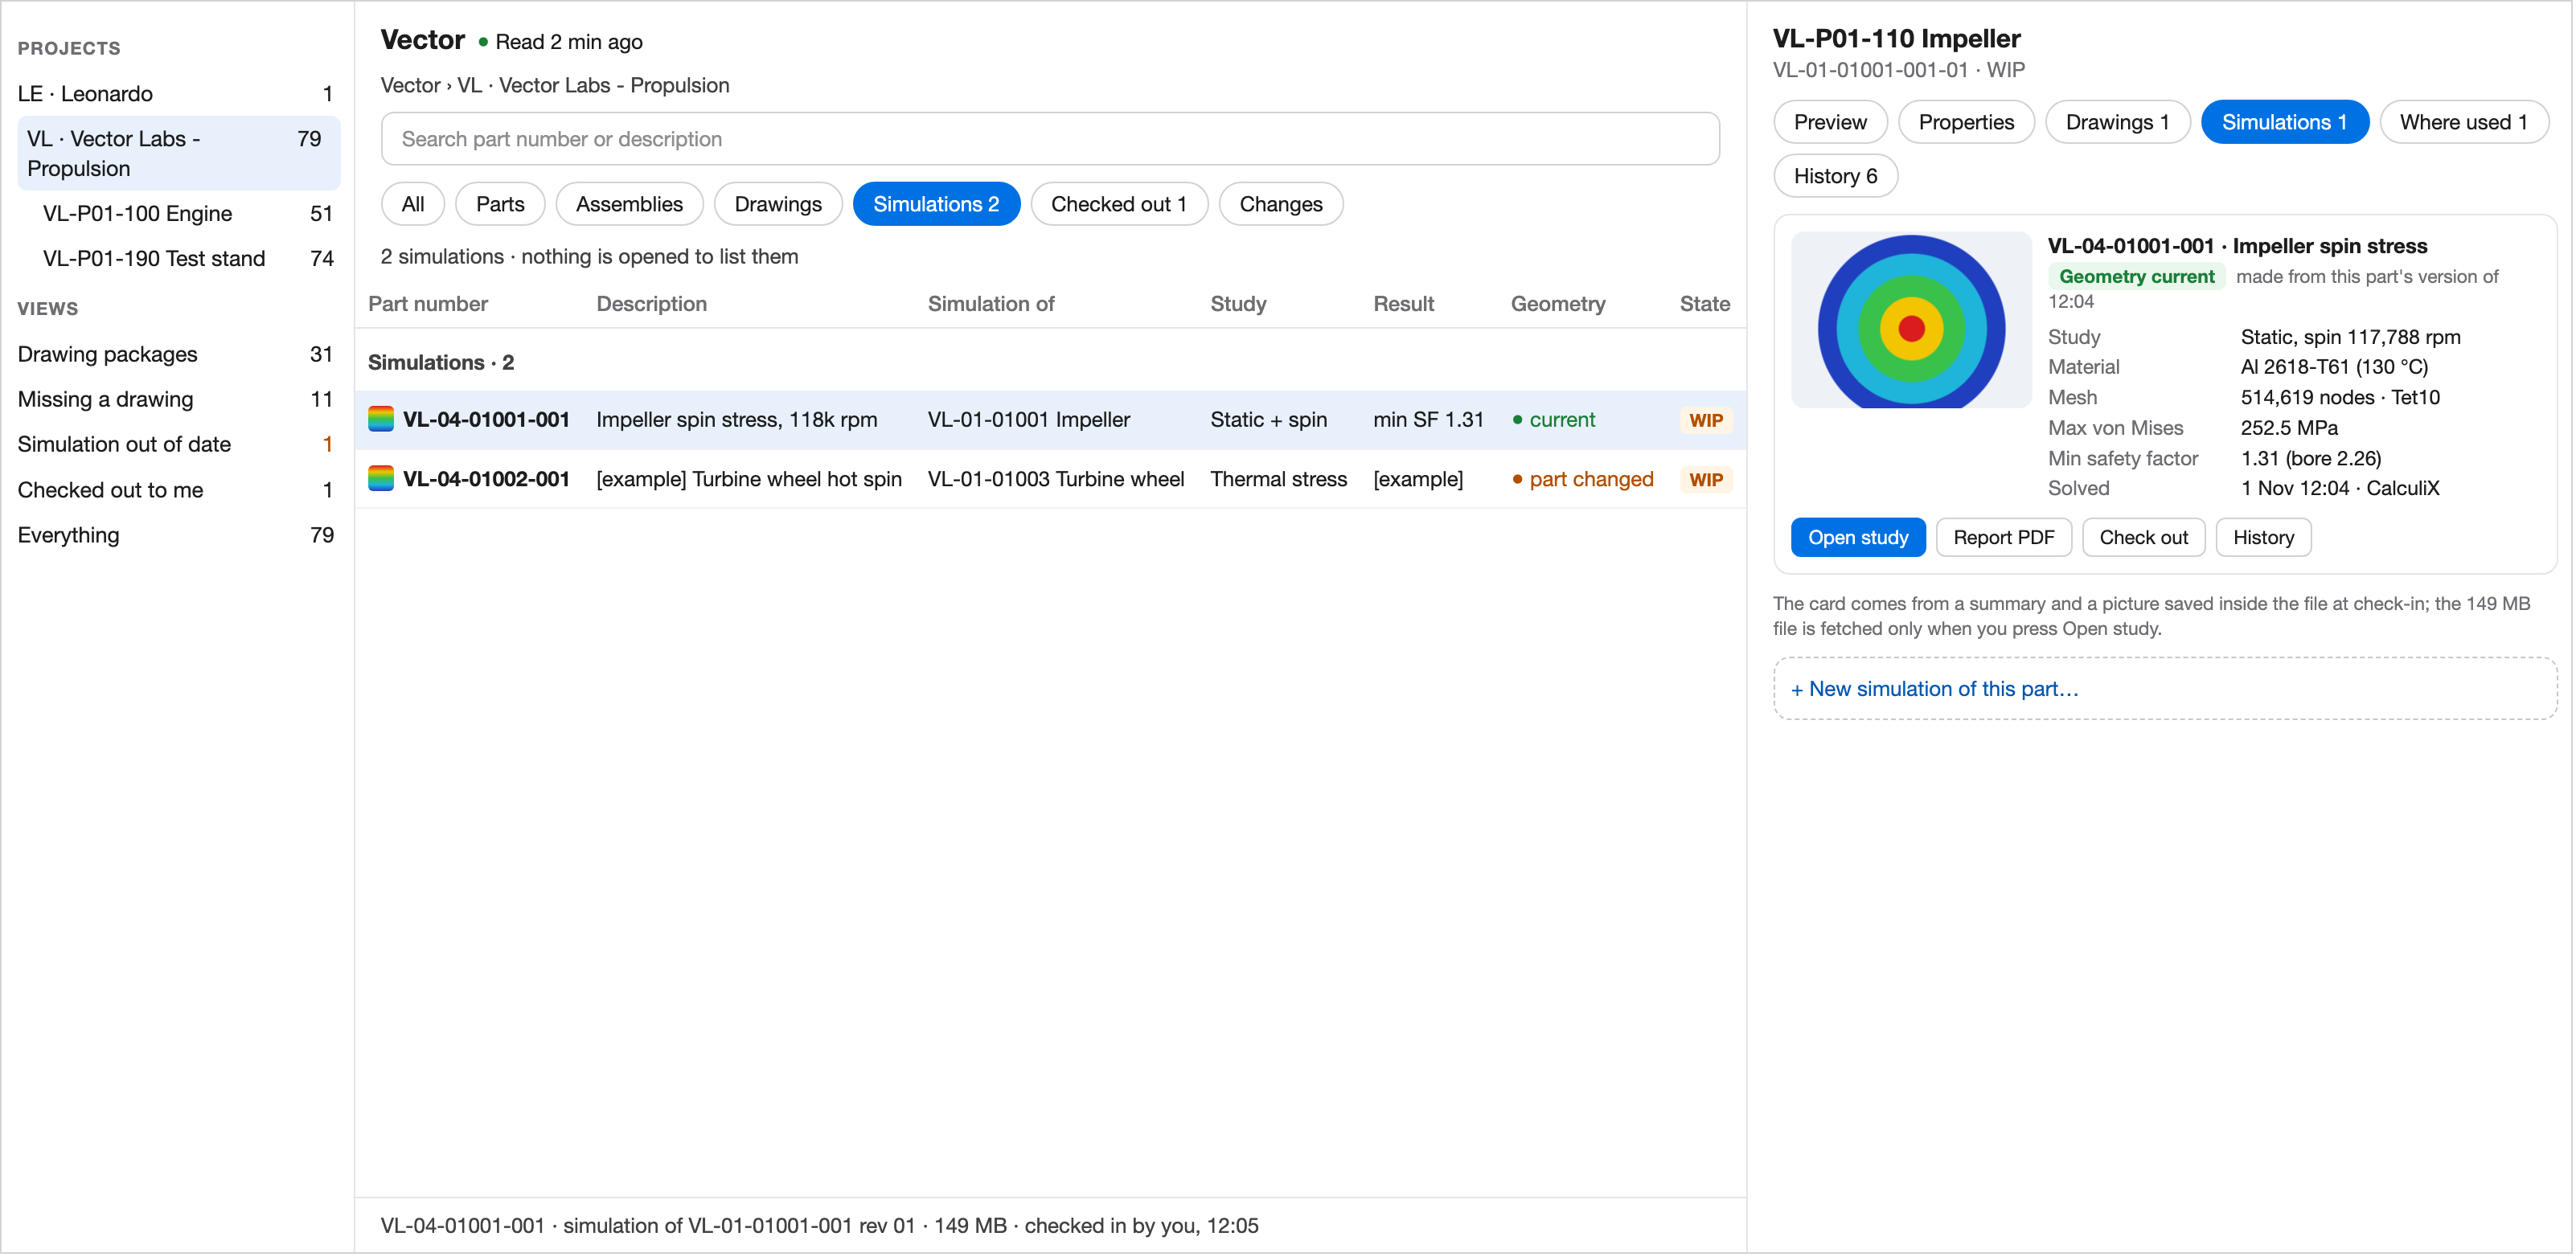
\includegraphics[width=\linewidth]{fig/pdm14_mockup.png}
\caption{Mockup: the Files list filtered to \emph{Simulations}, and the impeller's \emph{Simulations} tab. The card
(study, material, mesh, results, the picture) is read from inside the file; \emph{Open study} fetches the file. The
second row is an example of a simulation whose part changed after it was solved. The impeller numbers are the
Vector Jet session's of 1 Nov.}
\label{fig:pdm14-mockup}
\end{figure}

%----------------------------------------------------------------------
\subsubsection*{The proposal}

\paragraph{A simulation item.} A new item type \code{simulation} with its own document type, 04 \emph{Simulation}, so
the impeller study would be \code{VL-04-01001-001}. It carries \code{simulation\_of}, the part or assembly it analyses,
written and checked like \code{drawing\_of} and kept through a renumber. One part can have several simulations
(spin stress, modal, thermal). Simulations follow the same lifecycle as drawings: WIP, In Review, Released (read only),
Obsolete.

\paragraph{The file holds a copy of the geometry.} A study keeps its own copy of the solid, as the impeller study does
today, so its results always belong to the geometry they were solved on and opening it never pulls the part or its
links. At creation and at every check-in the vault records which version of the part the copy came from.

\paragraph{Is it still current?} The study is current when its copy matches the part's latest version. Comparing file
hashes would call a study out of date after any re-save of the part, even one that changes no geometry, so the test uses
the geometric fingerprint already built for SIM-07: for a solid $S$,
\[
  g(S)=H\bigl([V]_6,\ [A]_6,\ [\text{bbox}]_5,\ n_\text{faces},\ n_\text{solids}\bigr),
\]
where $[x]_k$ is $x$ to $k$ significant figures, $V$ the volume and $A$ the area (\code{geometry\_settings} in
\file{bruceworx\_sim\_model.py}). The part's fingerprint is written at
its check-in (with the picture and mesh); the study stores the fingerprint of the copy it was solved on. The study is
\emph{current} when $g_\text{part}=g_\text{study}$ and \emph{part changed} otherwise. A view \emph{Simulation out of
date} lists the second kind, as \emph{Missing a drawing} does for drawings.

\paragraph{Listing without opening.} At every save of a study file Heuretes FreeCAD writes three things into its zip: the
picture of the shown result, the light preview mesh, and a summary JSON (study type, solver, material, mesh size,
maximum stress and displacement, minimum safety factor, burst margin for spinning parts, the pre-check verdict, when it
was solved and the part fingerprint). The Files list, the part's \emph{Simulations} tab and the project tab read only
these. A 150\,MB file is copied to your Mac only when you open it, and the summary of an older version comes from the
cache keyed by its hash, as pictures do today.

\paragraph{Size.} Storage grows by the file size at every check-in:
\[
  \text{storage}\approx\sum_\text{studies} n_\text{versions}\cdot s_\text{file},
\]
so ten studies with five versions of 150\,MB are 7.5\,GB. Two changes keep that in hand: storing a version streams the
copy instead of reading the whole file into memory, and the solver work files (\file{.frd}, \file{.inp}, 248\,MB for
the impeller) never enter the vault; the results inside the \file{.FCStd} are the record. Question P4 asks whether to
go further.

\paragraph{Creating one.} \emph{New simulation of this part} on a part's \emph{Simulations} tab, and \emph{New Study}
in the Simulation workspace when the active document is a vault part, make the item, copy the solid into a new study
file and check it out to you. An existing file such as \file{VL-P01-110-SIM.FCStd} is brought in with \emph{Import} by
naming its part.

\paragraph{Release.} A simulation is not required to release a part. When a part being released has a simulation,
the release check adds a warning if it is \emph{part changed}, and the ECO can release the simulation with the part,
as it does a drawing. Study reports stay the release attachments they are today.

\paragraph{Projects.} Your mockup's \emph{Simulations} tab sits on a project page, which does not exist yet. Until
there are project pages, the same list is the Files list scoped to the project and filtered to Simulations
(figure~\ref{fig:pdm14-mockup}); the project tab becomes that list when project pages are built (question P7).

%----------------------------------------------------------------------
\subsubsection*{Phases}
\begin{enumerate}[nosep,label=P\arabic*.]
  \item \textbf{Item and link.} The \code{simulation} type, document type 04, \code{simulation\_of} in the journal, the
        renumber and the reference model; streamed storage. Tests in \file{addons/BruceWorx/tests}.
  \item \textbf{Summary inside the file.} Picture, mesh, summary JSON and the part fingerprint written at save and at
        check-in; the part's fingerprint written at its check-in.
  \item \textbf{Show them.} The \emph{Simulations} filter and columns in Files, the part's \emph{Simulations} tab, the
        \emph{Simulation out of date} view, the dashboard tile.
  \item \textbf{Make and bring in.} \emph{New simulation of this part}, New Study on a vault part, Import of an
        existing study file.
  \item \textbf{Release.} The release-check warning and the ECO releasing a simulation with its part.
\end{enumerate}
Every Heuretes FreeCAD copy that reads the vault must be updated before the first simulation is checked in, because an older
copy logs the new journal fields as unknown. On this Mac that is one app.

%----------------------------------------------------------------------
\subsubsection*{Questions for you}
\begin{enumerate}[label=P\arabic*.]
  \item \textbf{Own item.} A simulation is its own item with its own number (\code{VL-04-\ldots}), versions and lifecycle,
        rather than a file attached to the part's revision. \emph{Recommendation:} its own item, like drawings; a
        study is edited and re-solved on its own schedule.
  \item \textbf{Link field.} A new \code{simulation\_of} rather than reusing \code{drawing\_of}. \emph{Recommendation:}
        a new field; every reader of \code{drawing\_of} assumes a drawing.
  \item \textbf{Geometry.} The study keeps a copy of the solid (as today), with the part's fingerprint recorded, rather
        than linking to the part file. \emph{Recommendation:} the copy; results stay tied to what was solved, and
        opening a study never fetches the part.
  \item \textbf{Results in the vault.} Check in the whole file with its results (150\,MB a version), or offer
        \emph{Check in without results} for drafts (a few MB, re-solve to see fields). \emph{Recommendation:} whole
        file by default, solver work files never; add the light option only if the storage hurts.
  \item \textbf{Current or not.} Judge by the geometric fingerprint, not the file hash. \emph{Recommendation:} yes;
        a re-save of the part without a geometry change keeps the study current. Material or load changes in the
        part are not seen; the study owns those.
  \item \textbf{Release.} Not required for release; a warning when a released part's simulation is out of date; the
        ECO may release it with the part. \emph{Recommendation:} yes.
  \item \textbf{Project tab.} Build the project-scoped Simulations list in Files now and the project page tab with
        the project pages of your mockup, as their own epic. \emph{Recommendation:} yes; say if you want the project
        pages planned next.
  \item \textbf{Bring in the impeller study.} Import \file{VL-P01-110-SIM.FCStd} as \code{VL-04-01001-001}
        (simulation of the impeller) once P1--P3 are built, and point the Vector Jet session's script at the vault
        file. \emph{Recommendation:} yes, as the acceptance test.
  \item \textbf{Order.} After SIM-07 P1 is accepted and alongside SIM-07 P2. \emph{Recommendation:} yes; it shares
        the fingerprint and touches different files.
\end{enumerate}

\paragraph{Your answers (1 Nov).} P1, P2, P3 and P5 as recommended. \textbf{P4:} you choose at each check-in whether the
results go in (a \emph{Include results} box, remembered), until studies are made smaller. \textbf{P6:} no release
rule and no release warning; a part whose simulation is out of date gets a small bubble flag in the vault file
explorer. \textbf{P7:} the Simulations list goes on the project page, and the project pages of your mockup are built
now (\S\ref{sec:pdm15-plan}). \textbf{P8:} simulation files get their own extension, \file{.vlsim} (the same zip
inside; Heuretes FreeCAD opens and saves it, Finder opens it with Heuretes FreeCAD); the impeller study is imported as
\code{VL-04-01001-001}. \textbf{P9:} build now, without waiting for the SIM-07 acceptance; the UI can change once
everything is wired up. SIM-07 P2 starts at the same time.
